
% Inbuilt themes in beamer
\documentclass[aspectratio=169]{beamer}
\usepackage{graphicx}
% Theme choice:
\usetheme{CambridgeUS}

% Title page details: 
\title{Time Series} 
\author{John Green}
\date{April 2024}


\begin{document}

% Title page
\begin{frame}
    \titlepage 
\end{frame}

% Outline frame
\begin{frame}{Outline}
    \begin{enumerate}
       \item Notes on macroeconomic data
       \item Applications
       \item Lags
       \item Autocovariance and autocorrelation
       \item Forecasting
    \end{enumerate}
\end{frame}

\begin{frame}{Macroeconomic data}
    \begin{itemize}
       \item Volatility clustering
       \item Seasonal adjustments
       \item Data revisions and sources
       \item Unemployment rate 
       \item Labor force participation rate 
    \end{itemize}
\end{frame}

\begin{frame}{Uses of time series econometrics}
    Time series analysis is a highly valuable skill in industry:
    \begin{itemize}
       \item Forecasting (eg interest rates, returns to a stock, GDP growth)
       \item Dynamic treatment effects: impact of a policy after 1 month, 3 months, 2 years...
       \item Dynamic system analysis
    \end{itemize}
    But, we will have to deal with problems like correlation over time.
\end{frame}

\begin{frame}{Time series data}
    \begin{itemize}
       \item Generally similar to panel data, but with only one unit
       \item Takes the form $\{Y_t\}_{1 <= t <= T}$ with covariates $\{X_t\}_{1 <= t <= T}$
       \item For now, we assume timing is evenly spaced and there are no missing periods
    \end{itemize}
\end{frame}

\begin{frame}{Lags}
    \begin{itemize}
        \item Lags are very important in time series analysis
        \item $X_{t-1}$ is often a very good predictor of $X_{t}$
        \item More generally, the $j^{\text{th}}$ lag of $Y_t$ is $Y_{t-j}$
        \item We might take a difference: $\Delta_j Y_t = Y_{t} - Y_{t-j}$
    \end{itemize}
\end{frame}

% Outline frame
\begin{frame}{Log variables}
    \begin{itemize}
       \item Oftentimes we will use \textit{log} variables instead of the raw values
       \item Two benefits:
       \begin{itemize}
        \item Makes exponential growth linear
        \item Differences in logs are (approximately) equal to the percentage change:
        $$
        \log(1 + \alpha) \approx \alpha
        $$
        So long as $\alpha$ is ``small''
        \item So, $\log X_{t} - \log X_{t-1} = \log \dfrac{X_{t}}{X_{t-1}}$ is roughly the percentage change in $X$ from $t-1$ to $t$
       \end{itemize}
    \end{itemize}
\end{frame}

\begin{frame}{Autocorrelation}
    \begin{itemize}
       \item Just like with panel data, we will often have correlation between lagged values
       \item First autocovariance of $Y_t$: $cov(Y_t,Y_{t-1})$
       \item First autocorrelation of $Y_t$: $corr(Y_t,Y_{t-1}) \equiv \rho_1$
       \item Can calculate for any lag $j$ in the same way and get the $j^{th}$ serial correlation coefficient
    \end{itemize}
\end{frame}

\begin{frame}{Forecasting and stationarity}
    \begin{itemize}
       \item We will often be interested in making an out-of-sample (OOS) forecast of our variable
       \item This is similar to what we did before trying to target the oracle prediction
       \item We no longer care about causal interpretation of coefficients, OVB, etc.; we just want to get an accurate OOS prediction
       \item This requires that our data be \textit{stationary}
       \begin{itemize}
        \item Intuitively, our out-of-sample data needs to be similar to our sample Data
        \item Technically, we need the joint distribution across time to be independent of the time period we are looking at
       \end{itemize}
    \end{itemize}
\end{frame}

% \begin{frame}
%     \centering
%     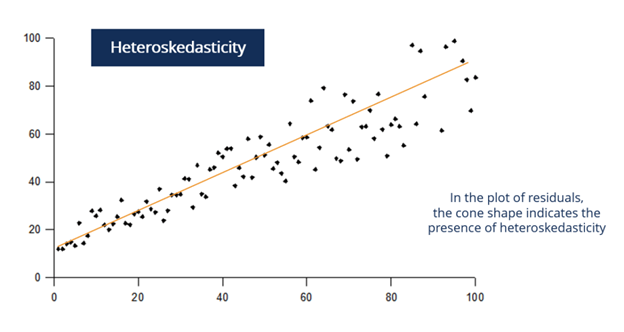
\includegraphics[width = .75\textwidth,keepaspectratio]{./figs/heteroskedasticity.png}
% \end{frame}

\end{document}